% libroResMat2
% Copyright (C) 2020  J.M. Perez Zerpa, et. al.
%
% This program is free software: you can redistribute it and/or modify
% it under the terms of the GNU General Public License as published by
% the Free Software Foundation version 3 of the License.
%
% This program is distributed in the hope that it will be useful,
% but WITHOUT ANY WARRANTY; without even the implied warranty of
% MERCHANTABILITY or FITNESS FOR A PARTICULAR PURPOSE. See the
% GNU General Public License for more details.
%
% You should have received a copy of the GNU General Public License
% along with this program.  If not, see <http://www.gnu.org/licenses/>.

\chapter{Análisis Seccional}

En esta unidad se presentan conceptos vinculados al análisis de tensiones en secciones transversales en vigas y/o columnas. %

En la Sección~\ref{sec:lnnc} se desarrolla y aplica un método práctico para el cálculo del Núcleo Central en secciones de cualquier forma. %
%
Parte del desarrollo es similar al usado en \citep{massood2001} mientras que otra parte fue desarrollada por los autores. %
%
Un desarrollo anterior se puede encontrar en el capítulo VIII de \citep{Timoshenko1953}. %
%
En la Sección~\ref{sec:nucleocentral} se presenta el análisis seccional para materiales que no soportan tracción, basado principalmente en el apartado 52 de \citep{Timoshenko1953} con una notación similar a la utilizada en los materiales de \textit{Resistencia de Materiales IIn} elaborados principalmente por el Prof. Atilio Morquio.

% -----------------------------------------------
% -----------------------------------------------
\section{Análisis Lineal de Secciones} \label{sec:lnnc}

En esta sección se presentan dos conceptos básicos en el análisis lineal de tensiones en secciones de elementos de viga: Línea Neutra (presentado en la Sección~\ref{sec:lineaneutra}) y Núcleo Central (presentado en la Sección~\ref{sec:nucleocentral}).

\subsection{Línea neutra} \label{sec:lineaneutra}

Se presenta a continuación una definición conceptual de Línea Neutra (LN).

\cajaconcepto{Definición: Línea Neutra}
{Sea una sección transversal de una viga sometida a esfuerzos de flexión, se define la \textbf{Línea Neutra} como el conjunto de puntos con \textbf{tensión axial nula}.}

La definición en términos de la función tensión puede ser enunciada como, que dada una sección transversal ubicada en un punto de coordenada $x$, la Línea Neutra es el conjunto de puntos $(y,z)$ que verifican: $\sigma(x,y,z) = 0$.

Existe una correspondencia biunívoca entre cada línea neutra y un punto de aplicación de la carga. %
%
A continuación se muestran los desarrollos para obtener la LN a partir del punto de aplicación y luego el desarrollo inverso.

\subsubsection{Determinación de la Línea Neutra a partir del punto de aplicación}


Se considera una viga con un corte en una sección tranversal en la posición $x$, y una carga $N$ aplicada en un punto de coordenadas $(y_A,z_A)$ como se muestra en la \autoref{fig:NCesquema1}. %

\begin{figure}[htb]
	\centering
	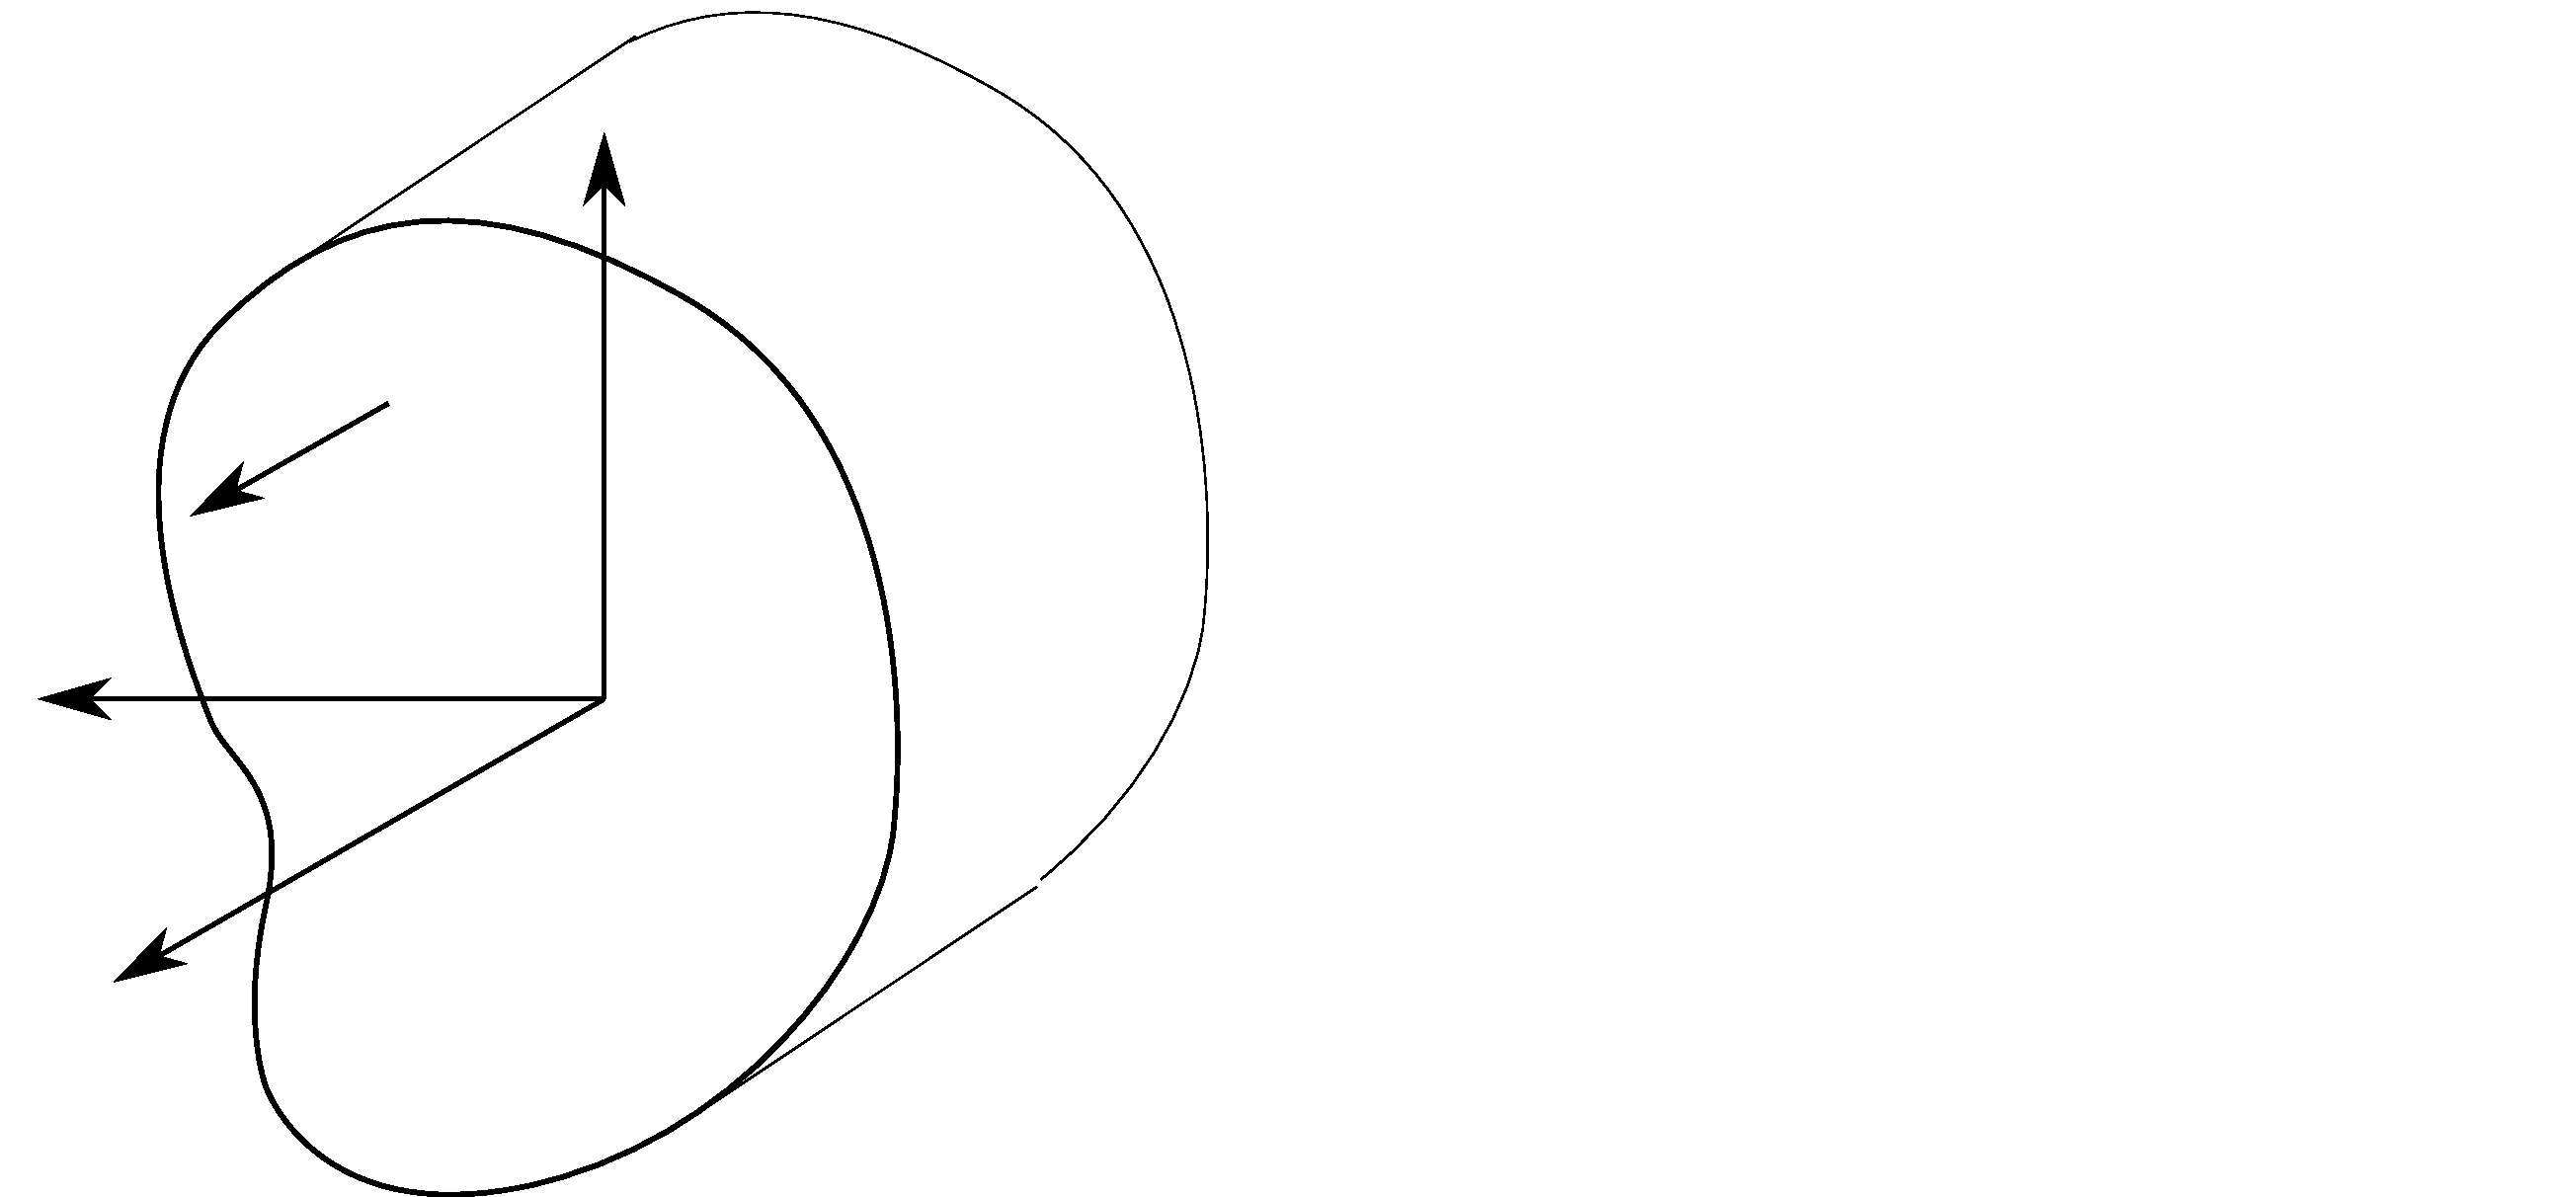
\includegraphics[width=0.5\textwidth]{NCesquema1}
	\caption{Esquema de sección y sistema de coordenadas considerado.}
	\label{fig:NCesquema1}
\end{figure}

Esta carga puede estar asociada tanto a cargas externas como a cargas internas producidas por el resto del elemento de viga. %
%
Se calcula el torsor equivalente en el baricentro de la sección, esto es, fuerza y momentos equivalentes:
%
\begin{equation}
N(x) = N, \qquad  M_z(x) = -N y_A \quad  \text{y} \quad M_y(x) = N z_A.
\end{equation}
%
Estas tres solicitaciones representan las solicitaciones internas correspondientes.


Sustituyendo las expresiones de las solicitaciones en la Ecuación~\eqref{eqn:tensaxiflexesv} y desarrollando se obtiene:
%
\begin{equation}
\sigma(x,y,z) = \frac{N(x)}{A}
\left(1 +  \frac{ y_A}{\rho_z^2} y +  \frac{ z_A}{\rho_y^2} z \right),
\end{equation}
%
donde fueron introducidas dos propiedades geométricas, llamadas radio de giro: $\rho_y = \sqrt{ I_y / A}$ y $\rho_z = \sqrt{ I_z / A}$. %
%
El desarrollo completo de este paso será visto en clase.

La condición de pertenencia a la LN es equivalente a anular la expresión de tensión axial. %
%
Por lo tanto, dado un punto de aplicación $(y_A,z_A)$, se demuestra que la ecuación de la LN es:
%
\begin{equation}\label{eqn:AptoLN}
\boxed{1 +  \frac{ y_A}{\rho_z^2} y +  \frac{ z_A}{\rho_y^2} z = 0}
\end{equation}

Se observa que la recta está contenida en el $plano$ $yz$ y no pasa por el origen, esto se debe a la existencia de una fuerza de directa aplicada.
%
En clase se discutirá con mayor detalle sobre esto.


\subsubsection{Determinación de punto de aplicación a partir de la Línea Neutra}

En esta sección se considera el caso en el cual se tiene una LN y se desea encontrar el punto de aplicación de la carga. %
%
Dada la ecuación de una recta genérica que no pasa por el origen:
$$
a y + b z +  c = 0,
$$
%
y usando que $(c\neq0)$ se obtiene la expresión:
%
\begin{equation}\label{eqn:ecrecta}
\frac{a}{c} y + \frac{b}{c} z +  1 = 0.
\end{equation}

Igualando los coeficientes de los polinomios de las expresión de las Ecuaciones \eqref{eqn:AptoLN} y \eqref{eqn:ecrecta} se tiene:
%
\begin{equation}
\boxed{y_A = \frac{a}{c} \rho_z^2
\qquad
z_A = \frac{b}{c} \rho_y^2}
\end{equation}

Dado que hay directa aplicada la recta que define la LN no pasa por el origen, por lo tanto se cumple que $c\neq0$.




% -------------------------------
\subsection{Núcleo central} \label{sec:nucleocentral}

Considerando una sección transversal cualquiera, se presenta una definición conceptual de Núcleo Central.

\cajaconcepto{Definición: Núcleo central}
{Se denomina Núcleo Central (NC) al lugar geométrico de los puntos del plano de la sección en los cuales una fuerza puntual de tracción (o compresión) aplicada generaría que toda la sección sea traccionada (o comprimida).}

Esto es equivalente a decir que, para cualquier punto de aplicación perteneciente al NC, la línea neutra correspondiente no corta a la sección.


\subsubsection{Cálculo de NC para secciones con borde suave}

El enfoque utilizado para el cálculo del NC es similar al utilizado en \citep{massood2001}. %
%

Se considera que el contorno de la sección transversal está dado por una curva paramétrica \textit{regular} y \textit{suave}. %
%
\begin{equation}
\mcC %
\left\{
\begin{array}{l}
y = y(t) \\
z = z(t) 
\end{array}
\right.
\end{equation}
donde las coordenadas $y$ y $z$ están medidas en el sistema de coordenadas locales.

La condición de regularidad implica que para todo parámetro $t$ se tiene que o bien $\dot{z}(t)\neq 0$ o $\dot{y}(t)\neq 0$, pero en ningún caso se cumple que $\dot{y}(t) = \dot{z}(t) = 0$. %
%
La condición de suavidad implica que tanto  $y(t)$ como $z(t)$ con funciones con derivada primera continua, es decir: de tipo $C^1$.

En la \autoref{fig:NCesquema2} se muestra un esquema de la sección transversal. %
%
En cada punto del contorno se puede definir una LN tangente, la cual se corresponderá con un punto de aplicación.

\begin{figure}[htb]
	\centering
	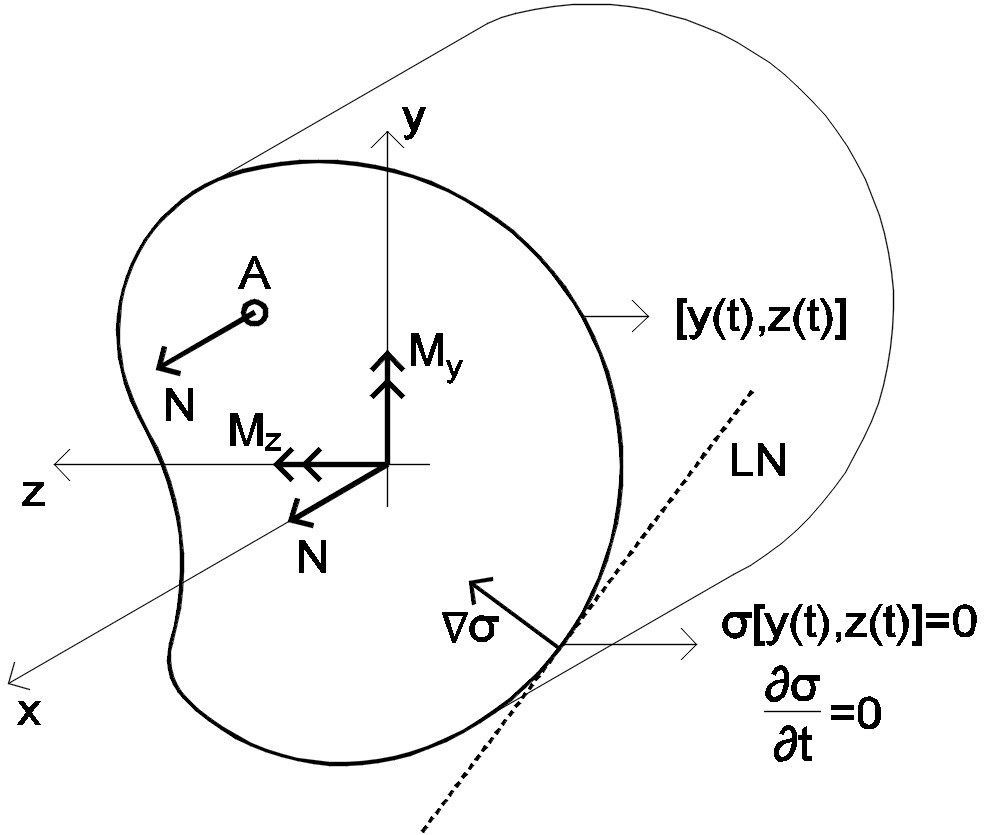
\includegraphics[width=0.5\textwidth]{NCesquema2}
	\caption{Esquema de sección y sistema de coordenadas considerado.}
	\label{fig:NCesquema2}
\end{figure}

Se desea obtener la curva paramétrica de los puntos de aplicación $(y_A(t),z_A(t))$, asociadas a las líneas neutras tangentes a la sección transversal en cada punto $y(t),z(t)$ y que no cortan a la sección. Por lo tanto, para dichos puntos de aplicación, existe al menos un punto del contorno de la sección correspondiente a la LN en que $\sigma(x,y(t),z(t)) = 0$. Utilizando la expresión de la Ecuación~\eqref{eqn:AptoLN} se tiene:
\begin{equation}\label{eqn:NC1}
1 +  \frac{ y_A(t)}{\rho_z^2} y(t) +  \frac{ z_A(t)}{\rho_y^2} z(t) = 0
\end{equation}

Se ha encontrado entonces un punto de aplicación $(y_A(t),z_A(t))$ en el que la expresión de tensión axial para los distintos puntos del contorno es,
\begin{equation}\label{eqn:NC1}
\sigma(x,y(\hat t),z(\hat t)) = \frac{N}{A} \left(1 +  \frac{ y_A(t)}{\rho_z^2} y(\hat t) +  \frac{ z_A(t)}{\rho_y^2} z(\hat t) \right)= 0
\end{equation}
Donde $\hat t$ es la variable que permite recorrer el contorno de la sección.

Los puntos del contorno de la sección, pertenecientes a la LN tangente a la sección y que no cortan a la misma, donde $\sigma(x,y(\hat t),z(\hat t)) = 0$, cumplen además que son puntos críticos, mínimo si $N(x)>0$ y máximo si $N(x)<0$. Imponiendo esta condición se obtiene:

\begin{equation}\label{eqn:NC2}
\frac{\partial \sigma}{\partial \hat t}(x,y(\hat t=t),z(\hat t=t)) = 0 = \frac{ y_A(t)}{\rho_z^2} \dot{y}(t) +  \frac{ z_A(t)}{\rho_y^2} \dot{z}(t)
\end{equation}

Combinando la Ecuación~\eqref{eqn:NC1} con la Ecuación~\eqref{eqn:NC2} y usando que $\mcC$ es regular y no pasa por el origen, se obtiene la curva paramétrica del borde del núcleo central:
%
\begin{eqnarray}
y_A(t) &=& - \frac{ \dot{z}(t) }{ \dot{z}(t) y(t) - \dot{y}(t) z(t) } \rho^2_z \label{eqn:ecsPSy} \\
z_A(t) &=& \frac{ \dot{y}(t) }{ \dot{z}(t) y(t) - \dot{y}(t) z(t) } \rho^2_y \label{eqn:ecsPSz}
\end{eqnarray}

Este planteo será desarrollado con mayor detalle en clase.

\subsubsection{Cálculo de NC para secciones con borde no suave}

En la \autoref{fig:NCesquema3} se muestra el esquema, en el $plano$ $yz$, de una sección con borde no suave para la cual, en el punto $R$ existe una discontinuidad en el vector tangente al borde. %
%
Esto provoca que las Ecuaciones \eqref{eqn:ecsPSy} y \eqref{eqn:ecsPSz} pierdan su validez.

\begin{figure}[htb]
	\centering
	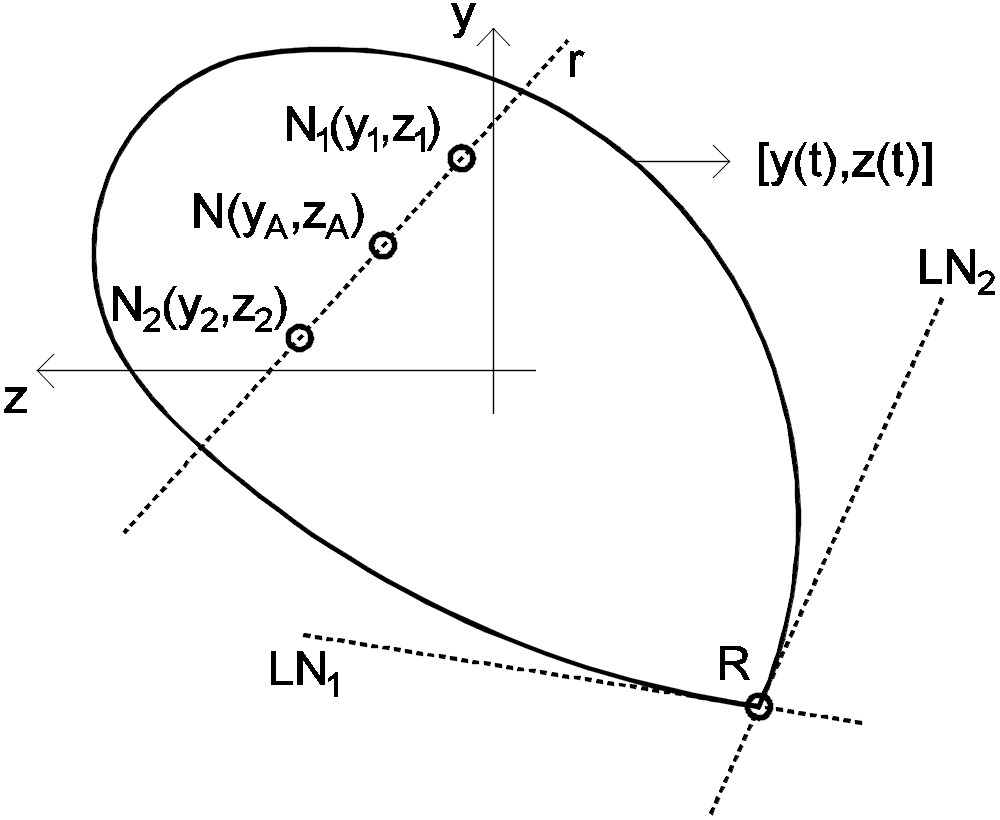
\includegraphics[width=0.5\textwidth]{NCesquema3}
	\caption{Esquema de sección en el plano.}
	\label{fig:NCesquema3}
\end{figure}

Se conoce que los puntos de aplicación $(y_1,z_1)$ y $(y_2,z_2)$ pertenecen al NC y tienen asociados las líneas neutras $LN_1$ y $LN_2$ respectivamente. La unión de los puntos de aplicación de las fuerzas de directa $N_1$ y $N_2$ forman una recta $r$, que se puede expresar como:
%
$$
r: z-z_1 = \frac{(z_1-z_2)}{(y_1-y_2)}(y-y_1).
$$

Desarrollando, factorizando y normalizando el término independiente, se obtiene:
%
\begin{equation}
\frac{y(z_1-z_2)-z(y_1-y_2)}{z_1y_2-y_1z_2}=1
\end{equation}

Se considera un nuevo punto de aplicación $(y_A,z_A)$ perteneciente a la recta $r$, por lo tanto para dicho punto se cumple que,
\begin{equation}
\frac{y_A(z_1-z_2)-z_A(y_1-y_2)}{z_1y_2-y_1z_2}=1,
\end{equation}
o también
\begin{equation}\label{eqn:suma}
\frac{ z_A y_2 - y_A z_2}{z_1y_2-y_1z_2} +
\frac{ y_A z_1 - z_A y_1}{z_1y_2-y_1z_2} =1,
\end{equation}

Por otra parte, la fuerza de directa $N$ actuando en este punto puede ser descompuesta en dos fuerzas de directa aplicadas simultáneamente en $(y_1,z_1)$ y $(y_2,z_2)$ respectivamente, se proponen las siguientes expresiones para dichas fuerzas,
%
\begin{equation}
N_1=N\frac{z_Ay_2-y_Az_2}{z_1y_2-y_1z_2}
\qquad
N_2=N\frac{y_Az_1-z_Ay_1}{z_1y_2-y_1z_2}
\end{equation}

Se demuestra que estas dos fuerzas de directa actuando simultáneamente tienen un torsor equivalente al de la fuerza $N$ aplicada en $(y_A,z_A)$.
%

La equivalencia en el momento $M_y$ es
\begin{equation}
M_y=N_1z_1+N_2z_2=Nz_A,
\end{equation}
%
sustituyendo las expresiones de $N_1$ y $N_2$ y desarrollando se obtiene el resultado esperado.
%
La equivalencia del momento $M_z$ es,
%
\begin{equation}
M_z=-(N_1y_1+N_2y_2)=-Ny_A,
\end{equation}
%
que es demostrada de forma análoga a la de $M_y$.
Y finalmente la  equivalencia de directas es:
\begin{equation}
N_1+N_2=N\frac{y_A(z_1-z_2)-z_A(y_1-y_2)}{z_1y_2-y_1z_2}=N,
\end{equation}
%
que es demostrada usando directamente la Ecuación~\ref{eqn:suma}.

Se tiene entonces que la fuerza de directa $N$ se puede escribir como una combinación lineal de las fuerzas de directa $N_1$ y $N_2$ de la forma:
$$
N=N_1+N_2=N(\lambda_1+\lambda_2)
$$
donde $\lambda_1$ y $\lambda_2$ son multiplicadores, que determinan la LN para la fuerza de directa N como una combinación de las LN de las fuerzas de directa $N_1$ y $N_2$, de la siguiente manera:
\begin{equation}
\lambda_1=\frac{z_Ay_2-y_Az_2}{z_1y_2-y_1z_2}
\qquad
\lambda_2=\frac{y_Az_1-z_Ay_1}{z_1y_2-y_1z_2}
\end{equation}

Tanto $N_1$ aplicada en $(y_1,z_1)$ como $N_2$ aplicada en $(y_2,z_2)$ producen tensiones axiales nulas en $R$ $(\sigma=0)$, por lo tanto la combinación lineal de ambas fuerzas de directa también produce tensiones axiales nulas en $R$. Lo anterior implica que si $N$ es aplicada en $(y_A,z_A)$ la LN correspondiente pasa por $R$. 

Para terminar de confirmar que los puntos $A$ en el segmento pertenecen al NC, es necesario mostrar que el haz de rectas LN definidas por toda carga aplicada en el segmento 1-2 es un haz que no corta la sección y es en particular el haz de rectas mostrado en la \autoref{fig:NCesquema4}.

\begin{figure}[htb]
	\centering
	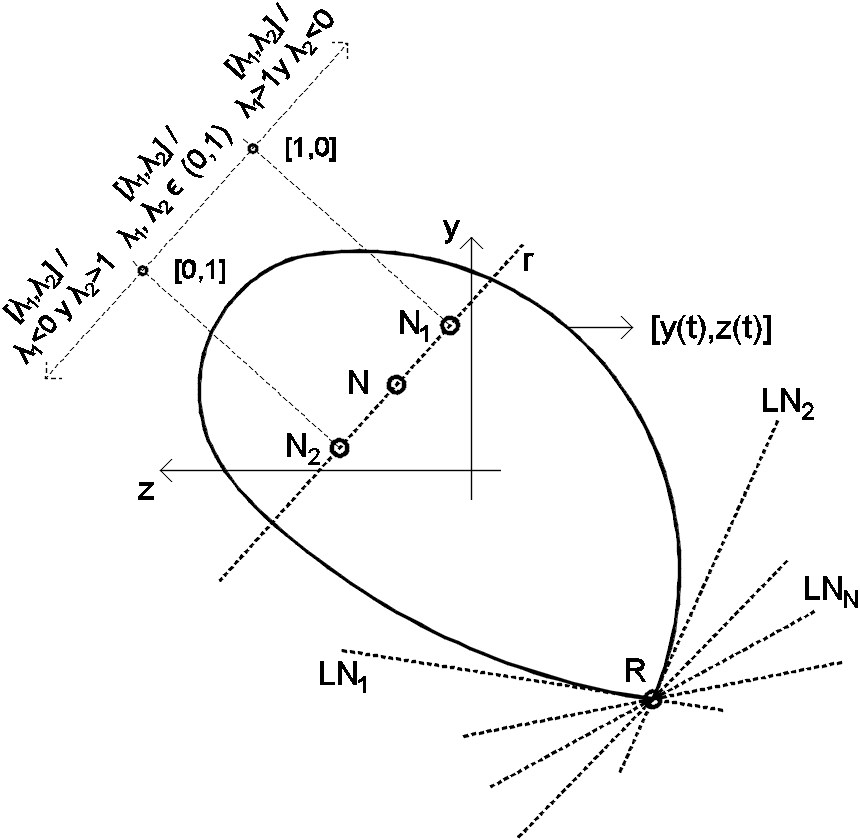
\includegraphics[width=0.6\textwidth]{NCesquema4}
	\caption{Esquema de sección en el plano.}
	\label{fig:NCesquema4}
\end{figure}


Para mostrar esto se considera la función de tensiones correspondiente a la aplicación de N en A:
%
\begin{equation}\label{eqn:sigmatotal}
\sigma = \frac{N}{A} \left( 1 + \frac{y_A}{\rho_z^2} y + \frac{z_A}{\rho_y^2} z \right).
\end{equation}

El vector gradiente es perpendicular a la LN y está dado por
$$
\nabla \sigma = \frac{N}{A} \left[ \begin{array}{c}
\displaystyle \dfrac{y_A}{\rho_z^2} \\[3mm]
\displaystyle \dfrac{z_A}{\rho_y^2}
\end{array} \right]
$$
Usando que 
$$
 y_A = \lambda_1 y_1 + \lambda_2 y_2 \quad \text{y} \quad 
 z_A = \lambda_1 z_1 + \lambda_2 z_2,
$$
y sustituyendo en la expresión del gradiente de $\sigma$ se tiene

\begin{equation}\label{eqn:gradiente}
\nabla \sigma = \frac{N}{A} \left( \lambda_1 \left[ \begin{array}{c}
\displaystyle \dfrac{y_1}{\rho_z^2} \\[3mm]
\displaystyle \dfrac{z_1}{\rho_y^2}
\end{array} \right]
+
\lambda_2 \left[ \begin{array}{c}
\displaystyle \dfrac{y_2}{\rho_z^2} \\[3mm]
\displaystyle \dfrac{z_2}{\rho_y^2}
\end{array} \right]
\right)
= 
\lambda_1 \frac{N}{A} \left[ \begin{array}{c}
\displaystyle \dfrac{y_1}{\rho_z^2} \\[3mm]
\displaystyle \dfrac{z_1}{\rho_y^2}
\end{array} \right]
+
\lambda_2 \frac{N}{A} \left[ \begin{array}{c}
\displaystyle \dfrac{y_2}{\rho_z^2} \\[3mm]
\displaystyle \dfrac{z_2}{\rho_y^2}
\end{array} \right].
\end{equation}


Por otra parte, se puede demostrar que si el punto $A$ está en el segmento 1-2, los valores $\lambda_1$ y $\lambda_2$ son ambos positivos. %
%
Usando esto en la Ecuación~\eqref{eqn:gradiente}, se ve que los vectores gradiente de tensión (perpendiculares a las $LN_N$ de la \autoref{fig:NCesquema4}), pueden ser escritos como combinación de los vectores fijos
$$
 \frac{N}{A} \left[ \begin{array}{c}
\displaystyle \dfrac{y_1}{\rho_z^2} \\[3mm]
\displaystyle \dfrac{z_1}{\rho_y^2}
\end{array} \right]
\quad \text{y} \quad 
 \frac{N}{A} \left[ \begin{array}{c}
\displaystyle \dfrac{y_2}{\rho_z^2} \\[3mm]
\displaystyle \dfrac{z_2}{\rho_y^2}
\end{array} \right].
$$
con multiplicadores positivos $\lambda_1$ y $\lambda_2$. Esto permite asegurar que todos los vectores gradiente estarán dentro de lo que se llama cono convexo\footnote{\href{https://en.wikipedia.org/wiki/Convex_cone}{https://en.wikipedia.org/wiki/Convex\_cone}}, y por lo tanto, dada la convexidad de la sección, se garantiza de que el haz de rectas no corta a la sección.

\subsection{Ejemplos}

\subsubsection{Sección elíptica}

En la Figura~\ref{fig:NCelip1} se tiene una sección regular de forma elíptica cuyo contorno responde a la siguiente curva paramétrica:

\begin{equation}
\mcC %
\left\{
\begin{array}{l} y(t)=Acos(t) \\ z(t)=Bsen(t) \end{array}
\qquad
\begin{array}{l} \dot{y}(t)=-Asen(t) \\ \dot{z}(t)=Bcos(t) \end{array}
\right.
\end{equation}

\begin{figure}[htb]
	\centering
\subfloat[Esquema de sección eliptica.]{
	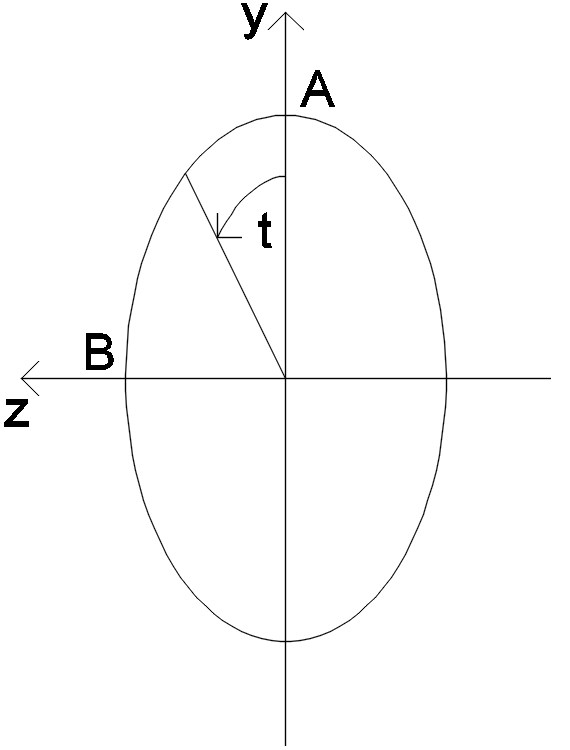
\includegraphics[width=0.35\textwidth]{NCelip1}
	\label{fig:NCelip1}}
\hspace{0.1\textwidth}
\subfloat[Núcleo central de sección eliptica.]{
	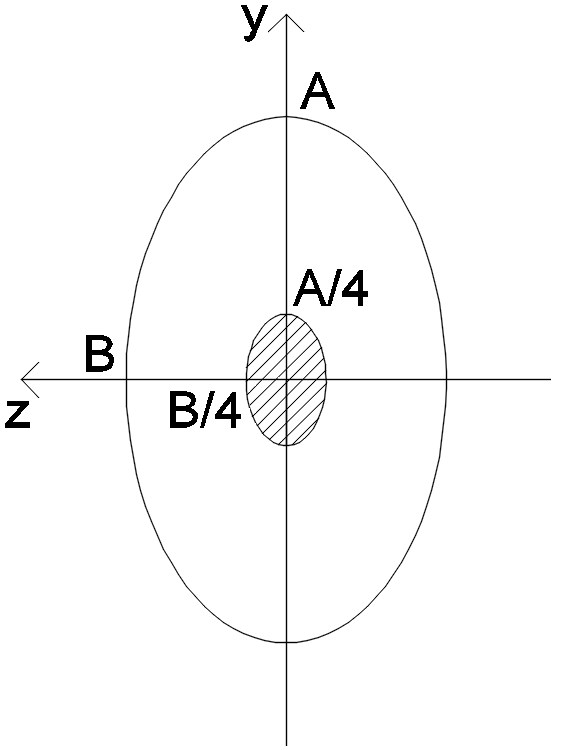
\includegraphics[width=0.35\textwidth]{NCelip2}
	\label{fig:NCelip2}}
\caption{Núcleo Central Sección Eliptica.}
	\label{fig:NCelip}
\end{figure}

Utilizando la Ecuación~\eqref{eqn:ecsPSy} y la Ecuación~\eqref{eqn:ecsPSz} se obtiene la curva paramétrica que describe al NC y que se indica en la Figura~\ref{fig:NCelip2}.
\begin{eqnarray}
y_A(t) &=& - \frac{A}{4} cos(t) \\
z_A(t) &=& - \frac{B}{4} sen(t)
\end{eqnarray}
Para el caso particular de una sección circular de radio $R$ se tiene que $A=B=R$, por lo tanto la curva paramétrica que describe al NC de una sección circular es:
\begin{eqnarray}
y_A(t) &=& - \frac{R}{4} cos(t) \\
z_A(t) &=& - \frac{R}{4} sen(t)
\end{eqnarray}

\subsubsection{Sección rectangular}

En la Figura~\ref{fig:NCrect1} se tiene una sección de forma rectangular de ancho $a$ y alto $b$. Se plantea la curva paramétrica correspondiente al lado superior de la sección como:

\begin{equation}
\mcC %
\left\{
\begin{array}{l} y(t)=b/2 \\ z(t)=t \end{array}
\qquad
\begin{array}{l} \dot{y}(t)=0 \\ \dot{z}(t)=1 \end{array}
\right.
\end{equation}

\begin{figure}[htb]
	\centering
\subfloat[Esquema de sección rectangular.]{
	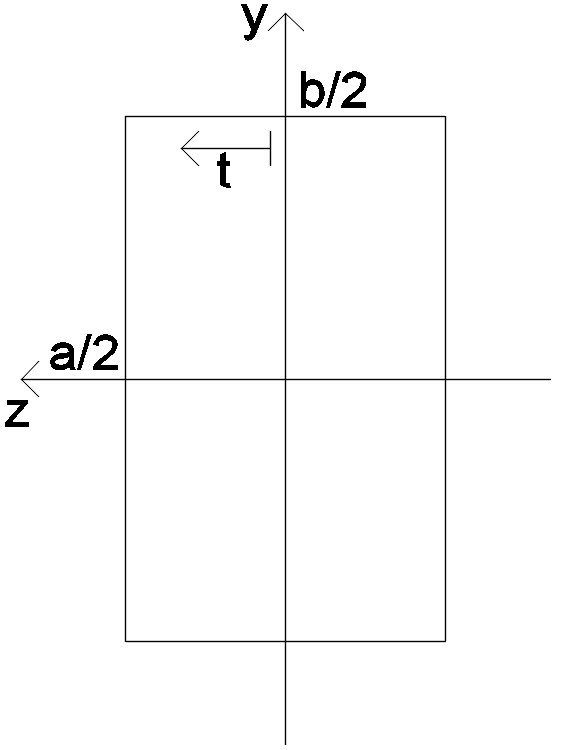
\includegraphics[width=0.35\textwidth]{NCrect1}
	\label{fig:NCrect1}}
\hspace{0.1\textwidth}
\subfloat[Núcleo central de sección rectangular.]{
	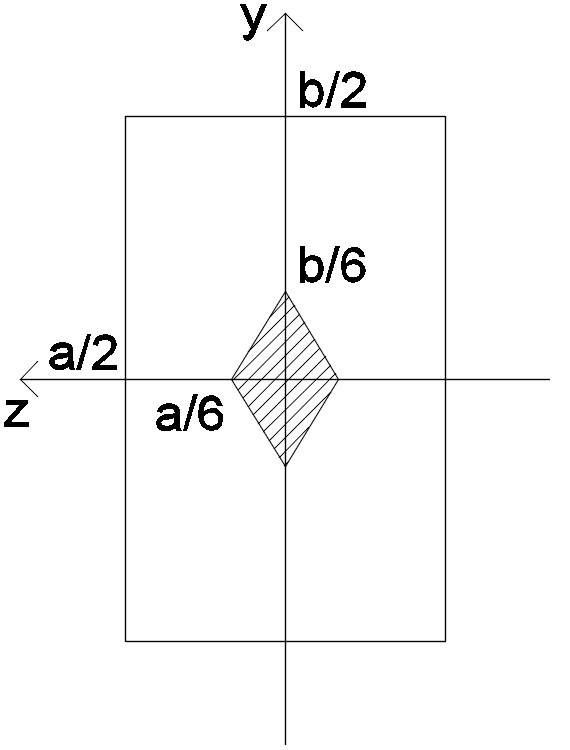
\includegraphics[width=0.35\textwidth]{NCrect2}
	\label{fig:NCrect2}}
\caption{Núcleo Central Sección Rectangular.}
	\label{fig:NCrect}
\end{figure}

Utilizando la Ecuación~\eqref{eqn:ecsPSy} y la Ecuación~\eqref{eqn:ecsPSz} se obtiene la curva paramétrica que describe al NC para el lado analizado,
\begin{eqnarray}
y_A(t) &=& - b/6 \\
z_A(t) &=& 0
\end{eqnarray}

Se observa que para el lado de la sección analizado, según lo esperado, se obtuvo un único punto de aplicación que describe dicho lado y que corresponde con la línea neutra para dicho punto de aplicación. Realizando un estudio análogo para cada lado, se obtienen los correspondientes puntos de aplicación que coinciden con los vértices del rombo indicado en la Figura~\ref{fig:NCrect2}.

Por otra parte, utilizando la propiedad demostrada para secciones no regulares, se tiene que los tramos de rectas que unen los puntos antes determinados pertenecen al NC. Por lo tanto, para una sección rectangular se obtiene el NC que se indica en la Figura~\ref{fig:NCrect2}.

Se observa que para determinar el NC en secciones no suaves, puede resultar conveniente determinar los puntos de aplicación que generan LN tangentes a la sección, en los puntos de discontinuidad de la misma, y utilizando la propiedad demostrada unir estos puntos mediante una recta.


% -----------------------------------------------
% -----------------------------------------------
\section{Análisis No Lineal de Secciones}

En esta sección se presentan los conceptos básicos en el análisis no lineal de tensiones en secciones, con particular interés en aquellos materiales que no soportan tracciones.

A partir de lo visto en la Sección~\ref{sec:nucleocentral} se conoce que, si se tiene una fuerza de directa en un punto de aplicación fuera del núcleo central, la línea neutra corta a la sección, teniendo una zona comprimida y otra traccionada. %
%
En el caso de materiales sin resistencia a tracción, como hormigón,  mampostería o fundaciones directas, el análisis no lineal de tensiones adquiere relevancia. %
%

\subsection{Materiales que no soportan tracción}

Se considera el caso, muy frecuente en la práctica, de sección simétrica y con el punto de aplicación de la fuerza de directa perteneciente al eje de simetría ($M_z=0$). Por otra parte se supondrá nula la tensión en la zona traccionada, y una relación líneal entre tensiones y deformaciones para la zona comprimida como muestra la Figura~\ref{fig:MNSTesquema}. Lo anterior implica que para la determinación del eje neutro no son válidas las ecuaciones obtenidas en la Sección~\ref{sec:lineaneutra}.

En la Figura~\ref{fig:MNSTesquema}, se define un sistema de coordenadas de forma tal que el origen del mismo es la intersección de la línea neutra con el eje de simetría de la sección y está orientado hacia la zona de mayores compresiones.

\begin{figure}[htb]
	\centering
\subfloat[Distribución de tensiones.]{
	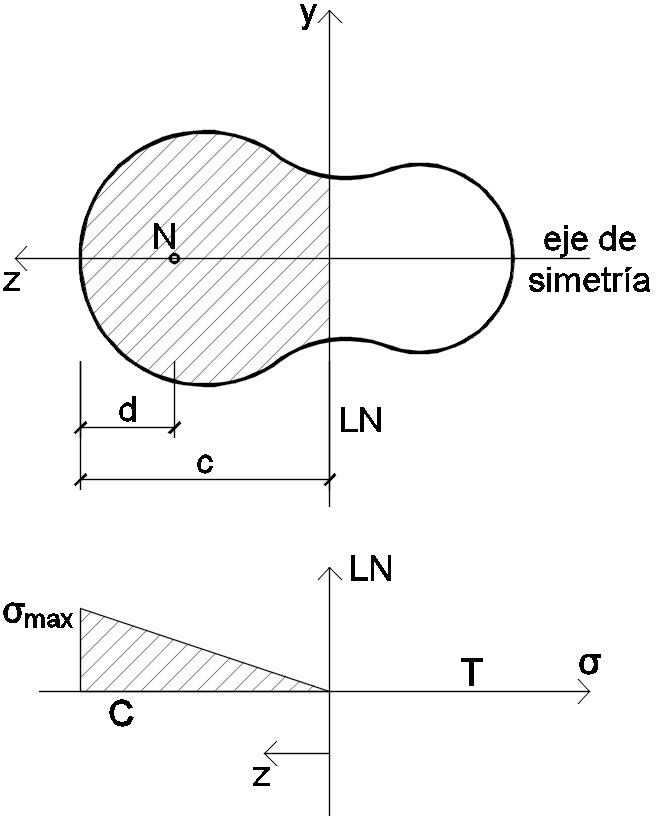
\includegraphics[width=0.4\textwidth]{MNSTesquema1}
	\label{fig:MNSTesquema1}}
\hspace{0.01\textwidth}
\subfloat[Distribución de deformaciones.]{
	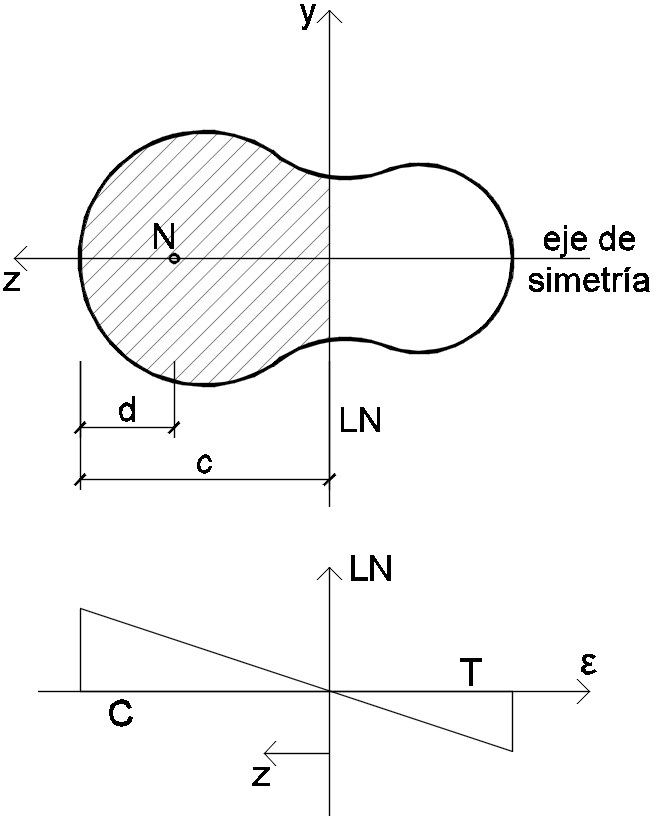
\includegraphics[width=0.4\textwidth]{MNSTesquema2}
	\label{fig:MNSTesquema2}}
\caption{Esquema de sección.}
	\label{fig:MNSTesquema}
\end{figure}

Se plantea el equilibrio de fuerzas en la dirección normal a la sección por lo que la resultante de las tensiones normales tendrá que ser igual a $N$,

\begin{equation}
N = \int_{A} \sigma (z) \dif A \label{eqn:ecseqN1},
\end{equation}
%
donde $A$ representa la región de la sección que está comprimida, es decir donde $\sigma$ es no nula.
% ---------------------

En la Figura~\ref{fig:MNSTesquema1} se observa que la distribución de tensiones es lineal y que $\sigma$ se puede escribir como,
\begin{equation}
\sigma(z) = kz = -\frac{\sigma_{max}}{c} z
\end{equation}

Sustituyendo en la Ecuación~\eqref{eqn:ecseqN1} se obtiene,
\begin{equation}
N = \int_{A} \sigma(z) \dif A=-\frac{\sigma_{max}}{c} \int_{A} z \dif A \label{eqn:ecseqN2}
\end{equation}

Por otra parte se plantea el equilibrio de momentos respecto del origen de coordenadas definido,
\begin{equation}
N(c-d) = \int_{A} \sigma(z) z \dif A = -\frac{\sigma_{max}}{c} \int_{A} z^2 \dif A \label{eqn:ecseqM}
\end{equation}

Se define la inercia de primer orden (o momento estático) referida a la línea neutra, que será función de la posición de la línea neutra $c$, como:
\begin{equation}
\int_{A} z \dif A = \mu_{LN}(c) \label{eqn:ecsI1}
\end{equation}

Se define también la inercia de segundo orden (o momento de inercia) referida a la línea neutra, que será función de la posición de la línea neutra $c$, como:
\begin{equation}
\int_{A} z^2 \dif A = I_{LN}(c) \label{eqn:ecsI2}
\end{equation}

Utilizando las Ecuaciones~\eqref{eqn:ecsI1} y~\eqref{eqn:ecsI2} en la Ecuaciónes~\eqref{eqn:ecseqN2} y~\eqref{eqn:ecseqM} respectivamente se tiene que,
\begin{eqnarray}
N &=& - \frac{\sigma_{max}}{c} \mu_{LN}(c)\label{eqn:ecsMNST1} \\
N(c-d) &=& - \frac{\sigma_{max}}{c} I_{LN}(c) \label{eqn:ecsMNST2}
\end{eqnarray}

Finalmente se realiza el cociente entre la Ecuación~\eqref{eqn:ecsMNST1} y la Ecuación~\eqref{eqn:ecsMNST2} y se obtiene que,
\begin{equation}
c-d = \frac{I_{LN}(c)}{\mu_{LN}(c)} \label{eqn:ecsMNST}
\end{equation}

En donde $c$ es la única incógnita a determinar.

\subsection{Ejemplo}

\subsubsection{Sección rectangular}

\begin{figure}[htb]
	\centering
	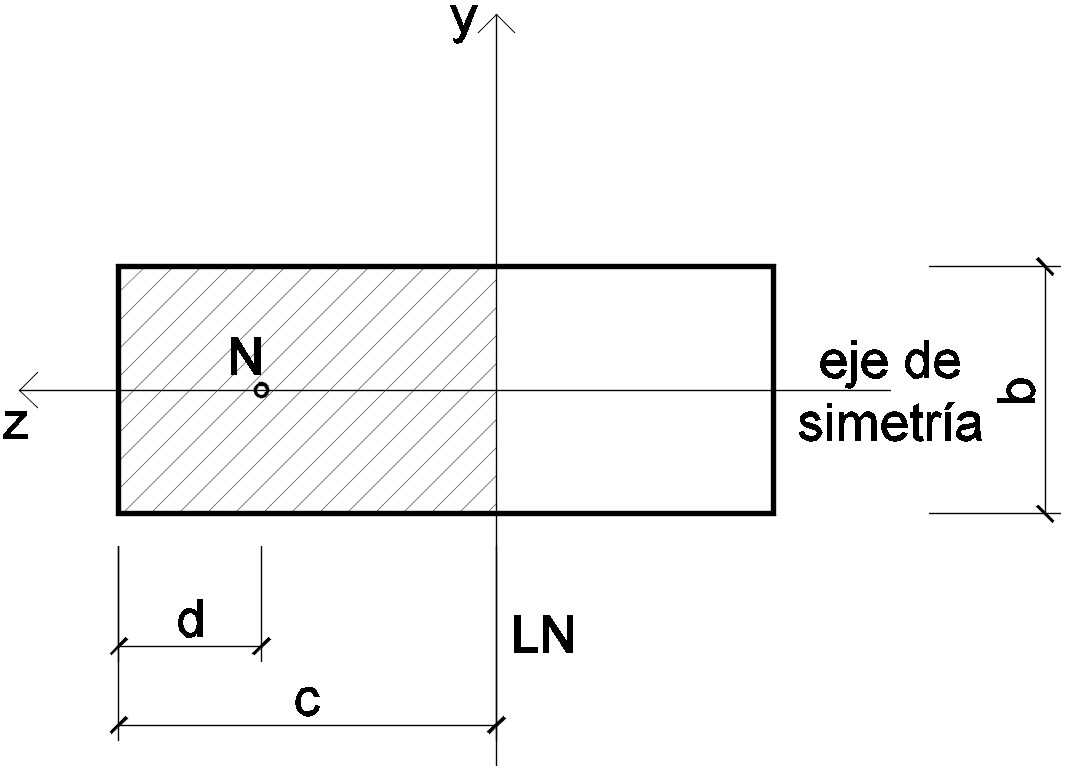
\includegraphics[width=0.5\textwidth]{MNSTrect}
	\caption{Sección rectangular.}
	\label{fig:MNSTrect}
\end{figure}

En primer instancia se determinan $I_{LN}(c)$ y $\mu_{LN}(c)$ de la siguiente manera,

\begin{equation}
I_{LN}(c) = \int_{A} z^2 \dif A = b \int_{0}^{c} z^2 \dif z = \frac{bc^3}{3} \label{eqn:ecsEjr1}
\end{equation}

\begin{equation}
\mu_{LN}(c) = \int_{A} z \dif A = b \int_{0}^{c} z \dif z = \frac{bc^2}{2} \label{eqn:ecsEjr2}
\end{equation}

Se tiene entonces que la relación entre el momento de segundo orden y el momento de primer orden es,
\begin{equation}
\frac{I_{LN}(c)}{\mu_{LN}(c)} = \frac{2}{3}c
\end{equation}

Utilizando la Ecuación~\eqref{eqn:ecsMNST} se tiene que,
\begin{equation}
c-d = \frac{2}{3}c
\end{equation}

Obteniendo que,
\begin{equation}
c = 3d
\end{equation}

Por otra parte utilizando la Ecuación~\eqref{eqn:ecsMNST1} se tiene que,
\begin{equation}
N = -\frac{\sigma_{max}}{c} \frac{bc^2}{2}
\end{equation}

Obteniendo que la tensión máxima de compresión es,
\begin{equation}
\boxed{
\sigma_{max} = -\frac{2N}{bc}
}
\end{equation}


\newpage

\section{Ejercicios}
\setcounter{ejercicio}{0}

\ejercicio 

La pieza de la figura soporta las cargas $P=30$ kN indicadas. Obtener el diagrama de tensiones normales en la sección $x-x$.

\begin{center}
  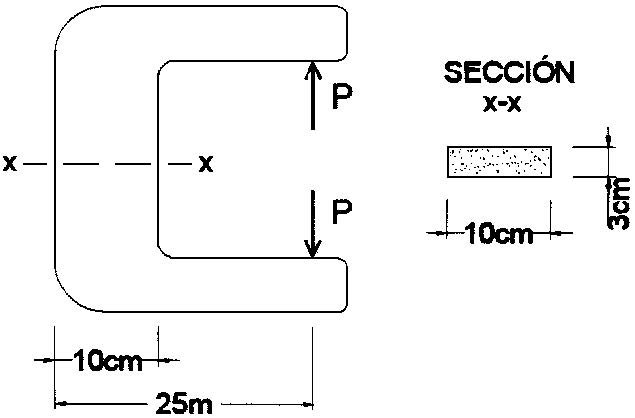
\includegraphics[width=0.5\linewidth]{UT6ej1}
\end{center}

\ejercicio 

\begin{minipage}[b]{0.55\textwidth}
Sobre la sección de la figura se aplican las cargas $P$ y $Q$ de compresión.

\parte Determinar los valores que deben tener los coeficientes $\alpha$ y $\beta$, tal que $\alpha P < Q < \beta P$, para que toda la sección esté comprimida.
\parte Para $Q= \alpha P$, determinar $P_{adm}$ si $a=20cm$ y $\sigma_{adm}=6MPa$. Obtener el diagrama de tensiones normales para ese valor hallado.
\end{minipage}
~
\begin{minipage}[b]{0.45\textwidth}
\begin{center}
	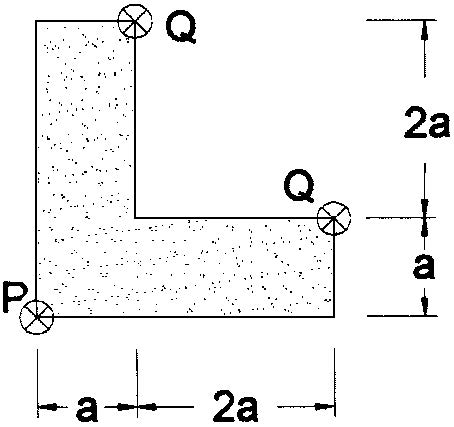
\includegraphics[width=0.6\linewidth]{UT6ej2}
\end{center}
\end{minipage}

\ejercicio 

%\begin{minipage}[t]{0.5\textwidth}
Una barra recta, formada por un perfil normalizado L $100x100x10$, de $3m$ de longitud, está empotrada en uno de sus extremos y sometida a su peso propio ($g=10 m/s^2$), como se muestra en la figura.

%\end{minipage}
%~
%\begin{minipage}{0.45\textwidth}

\begin{center}
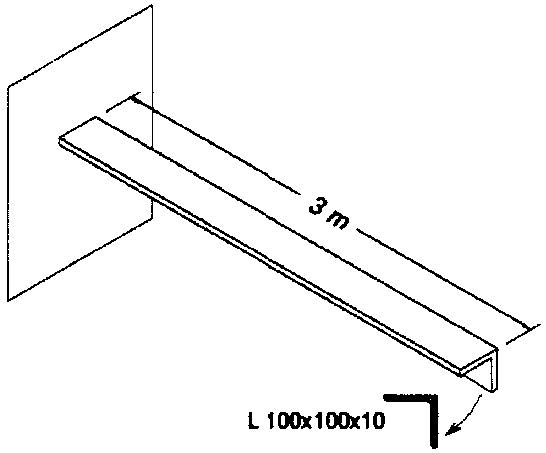
\includegraphics[width=0.45\linewidth]{UT6ej3}
\end{center}
%\end{minipage}

Se pide: determinar las máximas tensiones normales de tracción y compresión que se producen en la pieza.

\ejercicio 

Para la generación de columnas de iluminación se suelen emplear elementos prefabricados como los de la Figura~\ref{fig:UT64.1}. Se considera una de esas columnas de sección tubular de radio externo $R$ y radio interno $r= \alpha R$, como indica la Figura ~\ref{fig:UT64.2}.

\begin{figure}[htb]
	\centering
\subfloat[Elementos prefabricados]{
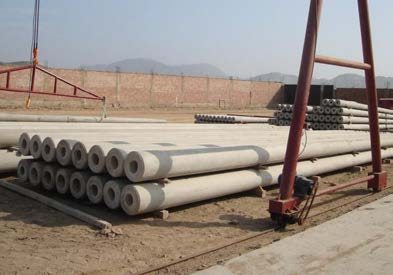
\includegraphics[width=0.37\textwidth]{UT6ej4-1}
	\label{fig:UT64.1}}
\hspace{0.1\textwidth}
\subfloat[Esquema de sección]{
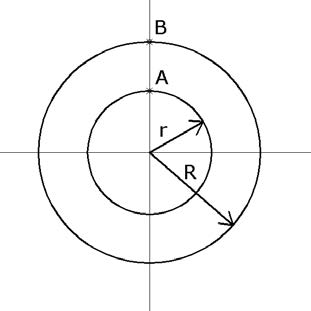
\includegraphics[width=0.27\textwidth]{UT6ej4-2}
	\label{fig:UT64.2}}
\caption{}
	\label{fig:UT64}
\end{figure}

\parte Determinar $\alpha$ para que el perímetro interior sea el contorno del núcleo central de la sección.
\parte Si se aplica una directa de compresión $P$ que varía de ubicación entre A y B, y el material es tal que $\sigma_{adm,trac}=9MPa$ y $\sigma_{adm,comp}=40MPa$, calcular $P_{adm}$ para $R=50cm$ y el $\alpha$ determinado.

\ejercicio 

En la Figura~\ref{fig:UT65.1} se presenta una viga pretensada de largo $L=25m$. El esquema básico de cálculo de la viga se presenta en la Figura~\ref{fig:UT65.2} y su sección se muestra en la Figura~\ref{fig:UT65.3}. Pretensar un elemento estructural implica introducirle esfuerzos previamente a su puesta en funcionamiento con el propósito de contrarrestar aquellos que serán ocasionados por la aplicación de las cargas que actuarán cuando ella entre en servicio. El pretensado de esta viga se puede representar mediante una fuerza concentrada $F$ de compresión en el eje vertical, a una cierta distancia $e$ del borde inferior.

\begin{figure}[htb]
	\centering
\subfloat[Elementos prefabricados]{
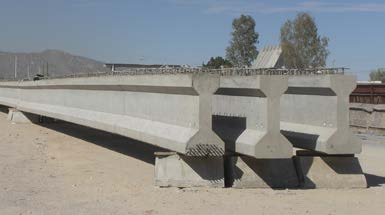
\includegraphics[width=0.3\textwidth]{UT6ej5-1}
	\label{fig:UT65.1}}
\hspace{0.1\textwidth}
\subfloat[Esquema básico de cálculo]{
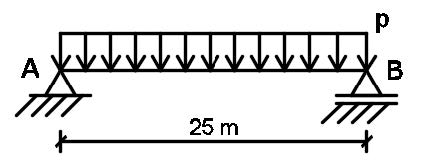
\includegraphics[width=0.4\textwidth]{UT6ej5-2}
	\label{fig:UT65.2}}
\caption{}
	\label{fig:UT65}
\end{figure}
\begin{figure}[htb]
	\centering
	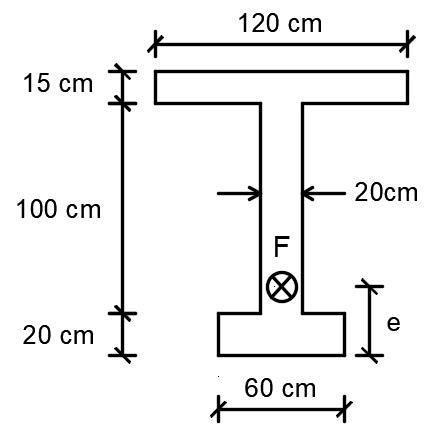
\includegraphics[width=0.35\textwidth]{UT6ej5-3}
	\caption{Esquema de sección.}
	\label{fig:UT65.3}
\end{figure}

\parte Determinar el núcleo central de la sección.
\parte Si $p=16 kN/m$ (incluido el peso propio), calcular la fuerza $F$ a aplicar y la excentricidad $e$, de manera que para la sección central de la viga se cumpla $\sigma_{sup}=0MPa$ y $\sigma_{inf}=18MPa$.

\ejercicio 

El esqquema de un mástil se representa en la Figura. Dicho mástil está construido en hormigón ($\rho=25 kN/m^3$), empotrado en su base y soporta en su extremo libre una fuerza horizontal $F$. Su sección transversal es constante y se indica en la Figura.

\begin{center}
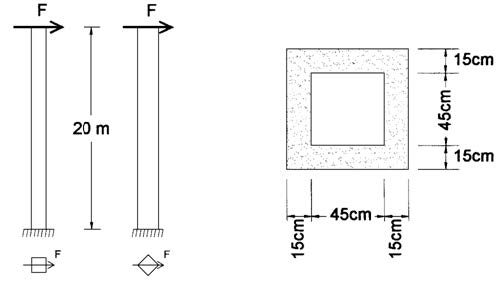
\includegraphics[width=0.7\linewidth]{UT6ej6}
\end{center}

\parte Determinar el núcleo central de la sección.
\parte Si la dirección de $F$ es paralela a una de las caras de la sección transversal, determinar su valor admisible para que no existan tensiones de tracción en el empotramiento. Trazar el diagrama de tensiones normales.
\parte Si la dirección de $F$ es paralela a una de las diagonales de la sección transversal, determinar su valor admisible para que no existan tensiones de tracción en el empotramiento. Trazar el diagrama de tensiones normales.
\parte Si la dirección de $F$ es paralela a una de las caras de la sección transversal, determinar su valor de modo que $\sigma_{trac,max}=-1/4\sigma_{comp,max}$. Trazar el diagrama de tensiones normales.

\ejercicio 

Sobre la sección de la figura se aplican las cargas $P$ y $Q$ de igual valor y signo. El punto de aplicación de P es fijo y coincide con el baricentro $G$, mientras que el de $Q$ se desplaza sobre el perímetro de la sección.

\begin{center}
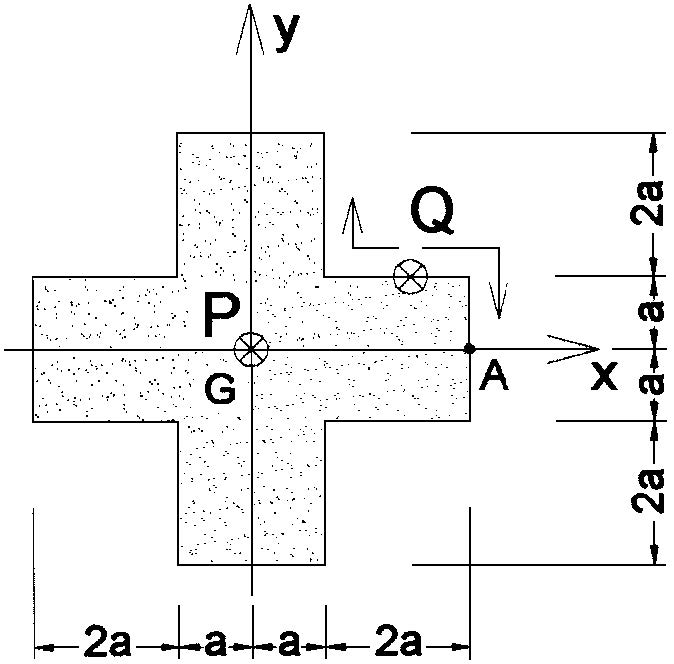
\includegraphics[width=0.4\linewidth]{UT6ej7}
\end{center}

\parte Determinar el núcleo central de la sección.
\parte Demostrar si existen o no posiciones de $Q$ para la cual las tensiones en la sección son todas de igual signo.
\parte Si $Q = \alpha P$ se aplica en A, determinar el máximo valor que puede tomar $\alpha$ para que el punto de aplicación de la resultante de las fuerzas esté dentro del núcleo central.

\ejercicio 

\begin{minipage}[b]{0.5\textwidth}
La zapata de la figura trasmite al terreno la descarga vertical de un pilar, siendo $P=40kN$.
Calcular el lado menor ($b$) de la zapata, si $\sigma_{terreno}=0,15MPa$.

\parte $e=0$.
\parte $e=0,25m$.
\parte $e=0,50m$.
\end{minipage}
~
\begin{minipage}[b]{0.5\textwidth}
\begin{center}
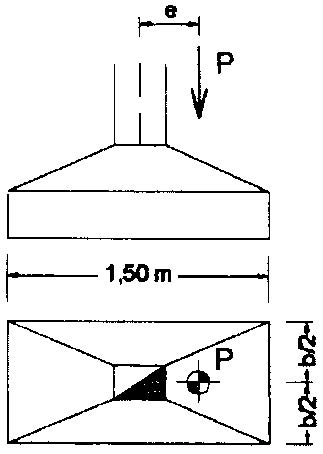
\includegraphics[width=0.45\linewidth]{UT6ej8}
\end{center}
\end{minipage}


\ejercicio 

La zapata de la figura trasmite al terreno la descarga vertical P cuyo punto de aplicación es el indicado en la figura.

Calcular $P_{adm}$ si $\sigma_{terreno}=0,6MPa$.

\begin{center}
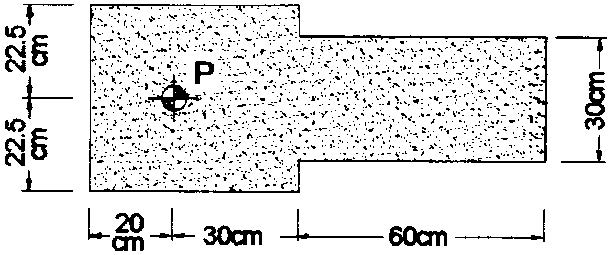
\includegraphics[width=0.5\linewidth]{UT6ej9}
\end{center}

\ejercicio (Adicional)

Se quiere construir un alero como el de la Figura~\ref{fig:UT610.1} según el esquema básico de cálculo de la Figura~\ref{fig:UT610.2}. Si $\sigma_{adm}=125MPa$, dimensionar en $PNI$ el travesaño BC.

\begin{figure}[htb]
	\centering
\subfloat[Alero]{

\includegraphics[width=0.35\textwidth]{UT6ej10-1}
	\label{fig:UT610.1}}
~
\subfloat[Esquema básico de cálculo]{
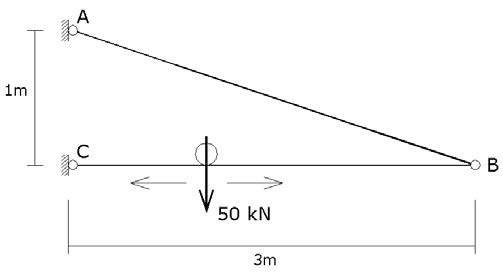
\includegraphics[width=0.55\textwidth]{UT6ej10-2}
	\label{fig:UT610.2}}
\caption{}
	\label{fig:UT610}
\end{figure}

\ejercicio (Adicional)

En la estructura de la Figura~\ref{fig:UT611.1} ($EI=cte$) el pilar AB descarga centrado en la zapata de hormigón de la Figura~\ref{fig:UT611.2}. Considerar $P=20kN$ y $L=2m$.

\begin{figure}[htb]
	\centering
\subfloat[Esquema básico de cálculo]{
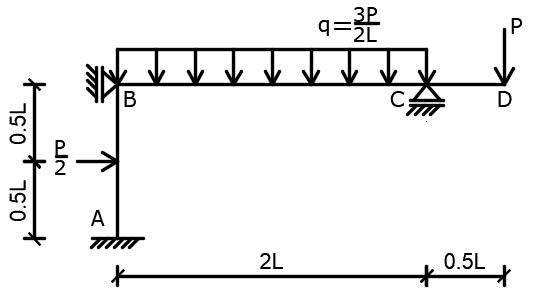
\includegraphics[width=0.5\textwidth]{UT6ej11-1}
	\label{fig:UT611.1}}
\hspace{0.1\textwidth}
\subfloat[Zapata]{
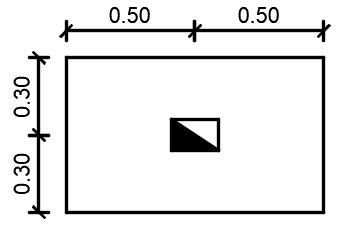
\includegraphics[width=0.3\textwidth]{UT6ej11-2}
	\label{fig:UT611.2}}
\caption{}
	\label{fig:UT611}
\end{figure}

\parte Obtener las reacciones de la estructura en el punto A.
\parte Determinar la máxima tensión en el terreno.
